\documentclass[12pt,a4paper,oneside]{report}

\usepackage[margin=0.9in,top=0.9in,bottom=0.9in]{geometry}
\usepackage[utf8]{inputenc}
\usepackage{lmodern}
\usepackage{amsmath,amssymb}
\usepackage{booktabs}
\usepackage{array}
\usepackage{fancyhdr}
\usepackage{float}
\usepackage{hyperref}
\usepackage{titlesec}
\usepackage{tikz}

\usetikzlibrary{
    arrows.meta,
    positioning,
    calc,
    shadows
}

% ================================================================
% SPACING
% ================================================================

\titleformat{\chapter}[display]
{\normalfont\LARGE\bfseries}
{\chaptertitlename\ \thechapter}
{3pt}
{\LARGE}

\titlespacing*{\chapter}{0pt}{-35pt}{12pt}
\titlespacing*{\section}{0pt}{10pt}{4pt}
\titlespacing*{\subsection}{0pt}{7pt}{3pt}

\setlength{\parindent}{0pt}
\setlength{\parskip}{4pt}

% ================================================================
% HEADER / FOOTER
% ================================================================

\pagestyle{fancy}

\fancyhf{}

\fancyhead[L]{\small\sffamily UCS503 - Software Engineering Project}
\fancyhead[R]{\small\sffamily ThaparTrade Prototype Report}

\fancyfoot[C]{\thepage}

\renewcommand{\headrulewidth}{0.4pt}

% ================================================================
% HYPERREF
% ================================================================

\hypersetup{
    colorlinks=true,
    linkcolor=black,
    citecolor=black,
    urlcolor=black
}

% ================================================================
% DOCUMENT
% ================================================================

\begin{document}

% ================================================================
% TITLE PAGE
% ================================================================

\begin{titlepage}

\centering

\vspace*{0.5cm}

{\Large\bfseries UCS503 -- Software Engineering Project}

\vspace{0.3cm}

{\large Academic Year 2026--2027}

\vspace{1.5cm}

{\Huge\bfseries
ThaparTrade: Campus Marketplace\\
for Student-to-Student Trading
}

\vspace{0.4cm}

{\large\itshape
A Structured Marketplace for Buying and Selling Products within the
Thapar Community
}

\vspace{2cm}

{\large\textbf{Submitted by:}}

\vspace{0.3cm}

\begin{tabular}{ll}

\textbf{1024030453} & Rajbir Singh \\

\textbf{1024030454} & Chitesh Jindal \\

\textbf{1024031095} & Ishan Garg \\

\end{tabular}

\vspace{0.5cm}

{\normalsize\textbf{B.E. Third Year, Computer Science \& Engineering}}

\vspace{1.6cm}

{\large\textbf{Submitted to:}}

\vspace{0.2cm}

{\large\textbf{Dr. Jeelani Asif}}

\vspace{0.1cm}

{\normalsize Department of Computer Science and Engineering}

\vspace{1.2cm}

\vfill

{\normalsize\textbf{Mid-Semester Evaluation Report}}

\vspace{0.15cm}

{\normalsize\textbf{Computer Science and Engineering Department}}

\vspace{0.1cm}

{\normalsize Thapar Institute of Engineering and Technology, Patiala}

\end{titlepage}

% ================================================================
% CONTENTS
% ================================================================

\pagenumbering{roman}

\tableofcontents

\newpage

\pagenumbering{arabic}

% ================================================================
% CHAPTER 1
% ================================================================

\chapter{Introduction}

\section{Background and Context}

Students at Thapar frequently buy and sell textbooks, cycles,
calculators, electronics, hostel items and other products within the
campus community. These transactions are commonly handled through
messaging groups, social media, personal contacts and word of mouth.

Such informal channels make listings difficult to discover and provide
no structured mechanism for searching, filtering or tracking
availability. ThaparTrade provides a centralized campus marketplace
where authenticated students can create, discover and manage product
listings.

\subsection{Problem Statement}

Existing student resale channels are fragmented and provide limited
search, filtering and listing management. Buyers cannot easily find
relevant products, while sellers lack a centralized platform for
managing listings and availability.

ThaparTrade resolves this gap through a campus-focused marketplace
where authenticated students can create, discover, manage and report
product listings.

\section{Project Objectives}

The core objectives of the ThaparTrade project comprise:

\begin{enumerate}

\item \textbf{User Authentication:}
Provide secure registration and login for students.

\item \textbf{Product Listing:}
Allow users to create, edit and delete product listings.

\item \textbf{Marketplace Discovery:}
Provide browsing, search and filtering of products.

\item \textbf{Listing Status:}
Maintain Available, Reserved and Sold product states.

\item \textbf{Reporting and Moderation:}
Allow users to report listings and administrators to review them.

\end{enumerate}

% ================================================================
% CHAPTER 2
% ================================================================

\chapter{Methodology and Design}

\section{System Architecture}

\subsection{High-Level Design}

ThaparTrade utilizes a modular three-tier architecture organized into
the Client Marketplace Layer, the Application Layer, and the Database
Layer. Figure~\ref{fig:architecture} illustrates the high-level
architecture.

% ================================================================
% ARCHITECTURE DIAGRAM
% ================================================================

\begin{figure}[H]

\centering

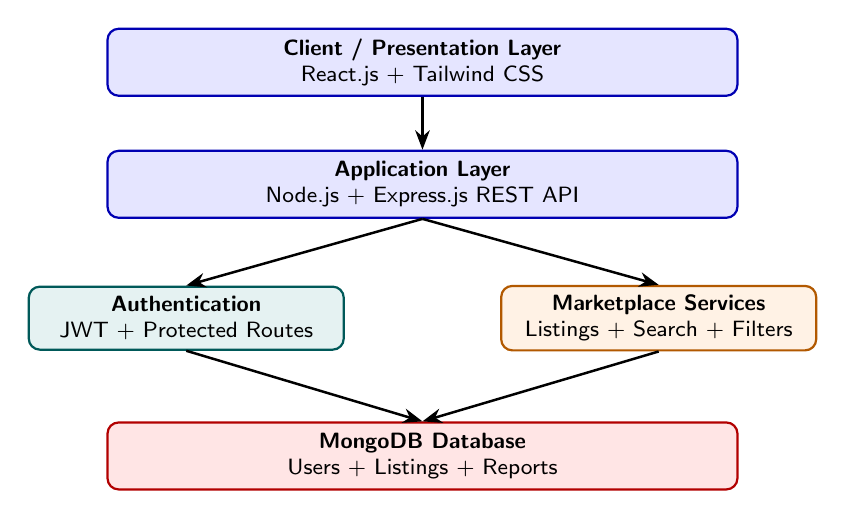
\begin{tikzpicture}[
    >=Stealth,
    every node/.style={
        font=\sffamily\footnotesize,
        align=center
    }
]

% Client box

\node[
    rectangle,
    rounded corners=4pt,
    draw=blue!70!black,
    line width=0.8pt,
    fill=blue!10,
    minimum width=8.0cm,
    minimum height=0.85cm
] (client) at (0,0)
{\textbf{Client / Presentation Layer}\\
React.js + Tailwind CSS};

% Application box

\node[
    rectangle,
    rounded corners=4pt,
    draw=blue!70!black,
    line width=0.8pt,
    fill=blue!10,
    minimum width=8.0cm,
    minimum height=0.85cm
] (application) at (0,-1.55)
{\textbf{Application Layer}\\
Node.js + Express.js REST API};

% Authentication

\node[
    rectangle,
    rounded corners=4pt,
    draw=teal!70!black,
    line width=0.8pt,
    fill=teal!10,
    minimum width=4.0cm,
    minimum height=0.8cm
] (authentication) at (-3.0,-3.25)
{\textbf{Authentication}\\
JWT + Protected Routes};

% Marketplace

\node[
    rectangle,
    rounded corners=4pt,
    draw=orange!70!black,
    line width=0.8pt,
    fill=orange!10,
    minimum width=4.0cm,
    minimum height=0.8cm
] (marketplace) at (3.0,-3.25)
{\textbf{Marketplace Services}\\
Listings + Search + Filters};

% Database

\node[
    rectangle,
    rounded corners=4pt,
    draw=red!70!black,
    line width=0.8pt,
    fill=red!10,
    minimum width=8.0cm,
    minimum height=0.85cm
] (database) at (0,-5.0)
{\textbf{MongoDB Database}\\
Users + Listings + Reports};

% Arrows

\draw[
    ->,
    line width=0.9pt
]
(client.south) -- (application.north);

\draw[
    ->,
    line width=0.9pt
]
(application.south) -- (authentication.north);

\draw[
    ->,
    line width=0.9pt
]
(application.south) -- (marketplace.north);

\draw[
    ->,
    line width=0.9pt
]
(authentication.south) -- (database.north);

\draw[
    ->,
    line width=0.9pt
]
(marketplace.south) -- (database.north);

\end{tikzpicture}

\caption{ThaparTrade High-Level Architecture}

\label{fig:architecture}

\end{figure}

% ================================================================
% TECHNICAL STACK
% ================================================================

\subsection{Technical Stack}

The implementation stack was selected for a practical full-stack web
application:

\begin{itemize}

\item \textbf{Frontend:} React.js and Tailwind CSS.

\item \textbf{Backend Runtime \& API:} Node.js and Express.js.

\item \textbf{Database \& Storage:} MongoDB.

\item \textbf{Authentication:} JSON Web Tokens (JWT).

\item \textbf{Image Storage:} AWS S3.

\item \textbf{Payment Integration:} Razorpay.

\item \textbf{Version Control:} GitHub.

\end{itemize}

% ================================================================
% IMPLEMENTATION
% ================================================================

\section{Implementation Details}

\subsection{Module 1: Authentication \& Product Listing}

Users register and log in before accessing protected marketplace
functionality. Authenticated users can create product listings with
title, category, description, price, condition and images. Users can
edit or delete their own listings and update product availability.

% ================================================================
% MODULE 1 DIAGRAM
% ================================================================

\begin{figure}[H]

\centering

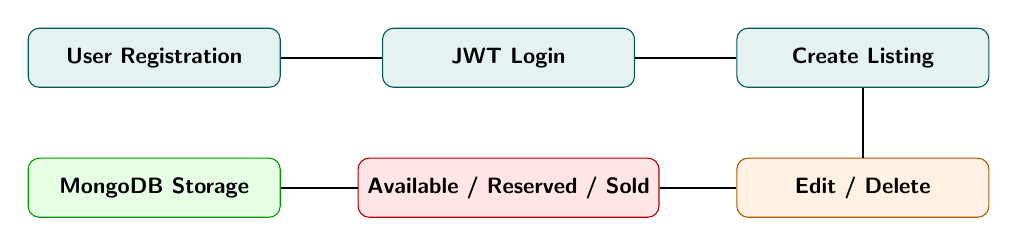
\begin{tikzpicture}[
    >=Stealth,
    every node/.style={
        font=\sffamily\footnotesize\bfseries,
        align=center
    }
]

% ------------------------------------------------
% TOP ROW
% ------------------------------------------------

\node[
    rectangle,
    rounded corners=4pt,
    draw=teal!70!black,
    fill=teal!10,
    minimum width=3.2cm,
    minimum height=0.75cm
] (m1a) at (0,0)
{User Registration};

\node[
    rectangle,
    rounded corners=4pt,
    draw=teal!70!black,
    fill=teal!10,
    minimum width=3.2cm,
    minimum height=0.75cm
] (m1b) at (4.5,0)
{JWT Login};

\node[
    rectangle,
    rounded corners=4pt,
    draw=teal!70!black,
    fill=teal!10,
    minimum width=3.2cm,
    minimum height=0.75cm
] (m1c) at (9,0)
{Create Listing};

% ------------------------------------------------
% BOTTOM ROW
% ------------------------------------------------

\node[
    rectangle,
    rounded corners=4pt,
    draw=green!60!black,
    fill=green!10,
    minimum width=3.2cm,
    minimum height=0.75cm
] (m1d) at (0,-1.65)
{MongoDB Storage};

\node[
    rectangle,
    rounded corners=4pt,
    draw=red!70!black,
    fill=red!10,
    minimum width=3.2cm,
    minimum height=0.75cm
] (m1e) at (4.5,-1.65)
{Available / Reserved / Sold};

\node[
    rectangle,
    rounded corners=4pt,
    draw=orange!70!black,
    fill=orange!10,
    minimum width=3.2cm,
    minimum height=0.75cm
] (m1f) at (9,-1.65)
{Edit / Delete};

% ------------------------------------------------
% HORIZONTAL CONNECTIONS
% ------------------------------------------------

\draw[
    line width=0.8pt
]
(m1a.east) -- (m1b.west);

\draw[
    line width=0.8pt
]
(m1b.east) -- (m1c.west);

\draw[
    line width=0.8pt
]
(m1d.east) -- (m1e.west);

\draw[
    line width=0.8pt
]
(m1e.east) -- (m1f.west);

% ------------------------------------------------
% VERTICAL CONNECTION
% ------------------------------------------------

\draw[
    line width=0.8pt
]
(m1c.south) -- (m1f.north);

\end{tikzpicture}

\caption{Authentication and Product Listing Flow}

\end{figure}

% ================================================================
% MODULE 2
% ================================================================

\subsection{Module 2: Marketplace \& Reporting}

Users can browse, search and filter marketplace listings. Users can
report problematic listings, after which an administrator can review
the report and remove or restore the listing.

% ================================================================
% MODULE 2 DIAGRAM
% ================================================================

\begin{figure}[H]

\centering

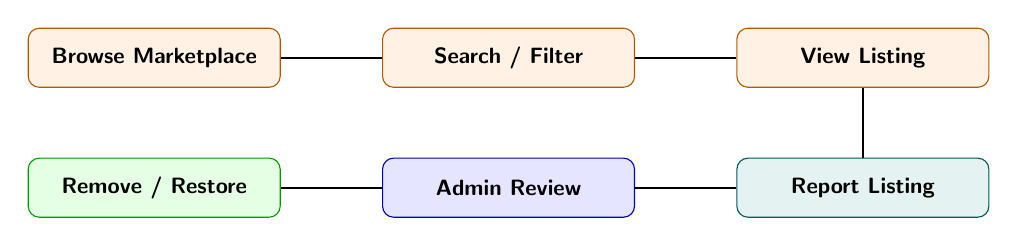
\begin{tikzpicture}[
    >=Stealth,
    every node/.style={
        font=\sffamily\footnotesize\bfseries,
        align=center
    }
]

% ------------------------------------------------
% TOP ROW
% ------------------------------------------------

\node[
    rectangle,
    rounded corners=4pt,
    draw=orange!70!black,
    fill=orange!10,
    minimum width=3.2cm,
    minimum height=0.75cm
] (m2a) at (0,0)
{Browse Marketplace};

\node[
    rectangle,
    rounded corners=4pt,
    draw=orange!70!black,
    fill=orange!10,
    minimum width=3.2cm,
    minimum height=0.75cm
] (m2b) at (4.5,0)
{Search / Filter};

\node[
    rectangle,
    rounded corners=4pt,
    draw=orange!70!black,
    fill=orange!10,
    minimum width=3.2cm,
    minimum height=0.75cm
] (m2c) at (9,0)
{View Listing};

% ------------------------------------------------
% BOTTOM ROW
% ------------------------------------------------

\node[
    rectangle,
    rounded corners=4pt,
    draw=green!60!black,
    fill=green!10,
    minimum width=3.2cm,
    minimum height=0.75cm
] (m2d) at (0,-1.65)
{Remove / Restore};

\node[
    rectangle,
    rounded corners=4pt,
    draw=blue!70!black,
    fill=blue!10,
    minimum width=3.2cm,
    minimum height=0.75cm
] (m2e) at (4.5,-1.65)
{Admin Review};

\node[
    rectangle,
    rounded corners=4pt,
    draw=teal!70!black,
    fill=teal!10,
    minimum width=3.2cm,
    minimum height=0.75cm
] (m2f) at (9,-1.65)
{Report Listing};

% ------------------------------------------------
% HORIZONTAL CONNECTIONS
% ------------------------------------------------

\draw[
    line width=0.8pt
]
(m2a.east) -- (m2b.west);

\draw[
    line width=0.8pt
]
(m2b.east) -- (m2c.west);

\draw[
    line width=0.8pt
]
(m2d.east) -- (m2e.west);

\draw[
    line width=0.8pt
]
(m2e.east) -- (m2f.west);

% ------------------------------------------------
% VERTICAL CONNECTION
% ------------------------------------------------

\draw[
    line width=0.8pt
]
(m2c.south) -- (m2f.north);

\end{tikzpicture}

\caption{Marketplace Discovery and Reporting Flow}

\end{figure}

% ================================================================
% CHAPTER 3
% ================================================================

\chapter{Results and Evaluation}

\section{Testing Methodology}

Testing followed a structured, multi-tier evaluation framework:

\begin{enumerate}

\item \textbf{Unit Testing:}
Individual testing of authentication, listing and search functionality.

\item \textbf{Integration Testing:}
End-to-end testing of REST APIs and MongoDB interactions.

\item \textbf{Scenario Validation:}
Validation across representative buyer, seller and reporting workflows.

\end{enumerate}

% ================================================================
% TESTING DIAGRAM
% ================================================================

\begin{figure}[H]

\centering

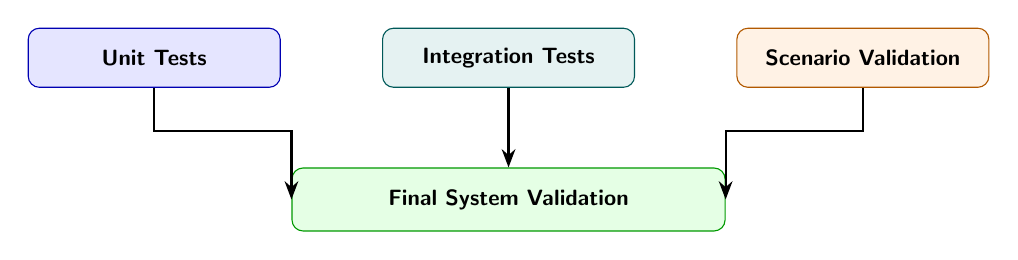
\begin{tikzpicture}[
    >=Stealth,
    every node/.style={
        font=\sffamily\footnotesize\bfseries,
        align=center
    }
]

% ------------------------------------------------
% TOP
% ------------------------------------------------

\node[
    rectangle,
    rounded corners=4pt,
    draw=blue!70!black,
    fill=blue!10,
    minimum width=3.2cm,
    minimum height=0.75cm
] (t1) at (0,0)
{Unit Tests};

\node[
    rectangle,
    rounded corners=4pt,
    draw=teal!70!black,
    fill=teal!10,
    minimum width=3.2cm,
    minimum height=0.75cm
] (t2) at (4.5,0)
{Integration Tests};

\node[
    rectangle,
    rounded corners=4pt,
    draw=orange!70!black,
    fill=orange!10,
    minimum width=3.2cm,
    minimum height=0.75cm
] (t3) at (9,0)
{Scenario Validation};

% ------------------------------------------------
% BOTTOM
% ------------------------------------------------

\node[
    rectangle,
    rounded corners=4pt,
    draw=green!60!black,
    fill=green!10,
    minimum width=5.5cm,
    minimum height=0.8cm
] (t4) at (4.5,-1.8)
{Final System Validation};

% ------------------------------------------------
% CONNECTIONS
% ------------------------------------------------

\draw[
    ->,
    line width=0.8pt
]
(t1.south) -- ++(0,-0.55) -| (t4.west);

\draw[
    ->,
    line width=0.8pt
]
(t2.south) -- (t4.north);

\draw[
    ->,
    line width=0.8pt
]
(t3.south) -- ++(0,-0.55) -| (t4.east);

\end{tikzpicture}

\caption{Multi-Tier Testing and Quality Assurance Framework}

\end{figure}

% ================================================================
% PERFORMANCE METRICS
% ================================================================

\section{Performance Metrics}

The prototype underwent functional evaluation to measure the
reliability of its core marketplace workflows. Table~\ref{tab:metrics}
summarizes the evaluation metrics.

\begin{table}[H]

\centering

\small

\begin{tabular}{lccc}

\toprule

\textbf{Evaluation Metric}
&
\textbf{Target Specification}
&
\textbf{Achieved}
&
\textbf{Status}
\\

\midrule

Listing Creation
&
Functional
&
Implemented
&
Achieved
\\

Search and Filtering
&
Functional
&
Implemented
&
Achieved
\\

Listing Status
&
Available / Reserved / Sold
&
Implemented
&
Achieved
\\

Reporting Workflow
&
Functional
&
Implemented
&
Achieved
\\

\bottomrule

\end{tabular}

\caption{ThaparTrade Prototype Performance Metrics Summary}

\label{tab:metrics}

\end{table}

\section{Analysis}

The prototype successfully implements the core student marketplace
workflow. Users can authenticate, create and manage product listings,
browse products and use search and filtering functionality.

The listing status mechanism provides clearer availability
information, while the reporting workflow provides a basic mechanism
for administrative moderation.

% ================================================================
% CHAPTER 4
% ================================================================

\chapter{Conclusion}

\section{Summary of Work}

During the first half of the project lifecycle, the team developed a
functional full-stack ThaparTrade prototype. The system demonstrates
user authentication, product listing management, marketplace
discovery, listing status management and reporting.

\section{Key Findings}

\begin{enumerate}

\item \textbf{Centralized Marketplace:}
A dedicated marketplace improves product discoverability.

\item \textbf{Structured Listings:}
Category, price and condition provide structured product information.

\item \textbf{Status Management:}
Available, Reserved and Sold states provide clearer availability.

\end{enumerate}

\section{Future Work and Recommendations}

For the final project phase, the team will implement:

\begin{enumerate}

\item Improved search and filtering.

\item Enhanced buyer-seller communication.

\item Marketplace notifications.

\item Enhanced administrative moderation.

\end{enumerate}

\section{Final Remarks}

ThaparTrade offers a practical campus marketplace for student-to-student
trading. The prototype establishes the core workflow for authenticated
users, product listings, marketplace discovery, availability management
and reporting.

\end{document}
